\section{Poisson solver}
\label{sec:poisson}
\renewcommand{\thesubsection}{\thesection.\arabic{subsection}}
In this section of the lab report, we will dicuss a prallel implementation of the Poisson solver. The Poisson solver is a numerical method used to solve the Poisson equation, which is a partial differential equation that is useful in many areas of physics. \\
\textbf{Note:} For local testing and development I'll run the code with \texttt{mpirun} instead of the \texttt{srun} command on the cluster. \\

\subsection{Building a parallel Poisson solver}
For the first part of the exercise we follow the steps lined out in the assignment sheet. I'll comment on the steps 1 through 10 and related questions bellow. The finished implementation can be found in the appendix for this section. \\
\begin{enumerate}
    \item \textbf{Step:} After adding MPI\_Init and MPI\_Finalize, we can run the program with multiple processes. We can see that the program runs with 4 processes in \autoref{fig:poisson_step1} via the quadrupeled output.
    \begin{figure}[H]
        \centering
        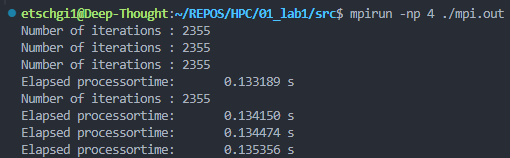
\includegraphics[width=0.5\textwidth]{../fig/lab1/step1.png}
        \caption{MPI\_Poisson after Step 1 - Running with 4 processes}
        \label{fig:poisson_step1}
    \end{figure}
    \item \textbf{Step:} To see which process is doing what, I included the rank of the process for the print statements as shown in \autoref{fig:poisson_step2}.
    \begin{figure}[H]
        \centering
        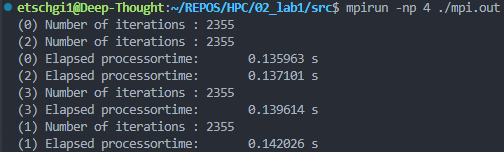
\includegraphics[width=0.5\textwidth]{../fig/lab1/step2.png}
        \caption{MPI\_Poisson after Step 2 - Running with 4 processes}
        \label{fig:poisson_step2}
    \end{figure}
    \item \textbf{Step:} Next we define \texttt{wtime} as a global double and replace the four utility timing functions with the ones given on Brightspace. A quick verification as shown in \autoref{fig:poisson_step3} shows that the program still runs as expected.
    \begin{figure}[H]
        \centering
        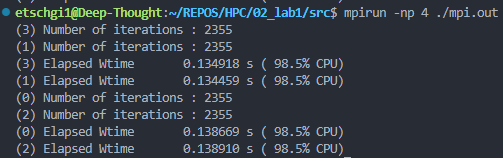
\includegraphics[width=0.5\textwidth]{../fig/lab1/step3.png}
        \caption{MPI\_Poisson after Step 3 - Running with 4 processes}
        \label{fig:poisson_step3}
    \end{figure}
    \item \textbf{Step:} Next we check if two processes indeed give the same output. Both need 2355 iterations to converge and the \texttt{diff} command returned no output, which means that the files content is identical. 
    \item \textbf{Step:} Now only the process with rank 0 will read data from files and subsequently broadcast it to the others. 
\end{enumerate}